\documentclass{article}

% if you need to pass options to natbib, use, e.g.:
% \PassOptionsToPackage{numbers, compress}{natbib}
% before loading nips_2017
%
% to avoid loading the natbib package, add option nonatbib:

\PassOptionsToPackage{numbers, compress}{natbib}
\usepackage[final]{nips_2017}

% to compㅁle a camera-ready version, add the [final] option, e.g.:
\usepackage[utf8]{inputenc} % allow utf-8 input
\usepackage[T1]{fontenc}    % use 8-bit T1 fonts
\usepackage{hyperref}       % hyperlinks
\usepackage{url}            % simple URL typesetting
\usepackage{booktabs}       % professional-quality tables
\usepackage{amsfonts}       % blackboard math symbols
\usepackage{nicefrac}       % compact symbols for 1/2, etc.
\usepackage{microtype}      % microtypography
\usepackage{amsmath, amssymb, amsfonts, amsthm}
\usepackage[export]{adjustbox}
\usepackage{subcaption}
\usepackage[font=small]{caption}
\usepackage{todonotes}
%\usepackage[]{algorithm2e}
\usepackage{algorithm}
\usepackage[noend]{algpseudocode}

% Some reference styles
\newcommand{\eref}[1]{(\ref{#1})}% Equation
\newcommand{\aref}[1]{Algorithm~\ref{#1}}% Algorithm
\newcommand{\sref}[1]{Section~\ref{#1}}% Section
\newcommand{\figref}[1]{Figure~\ref{#1}}% Figure
\newcommand{\tabref}[1]{Table~\ref{#1}}% Table

\DeclareMathOperator*{\argmax}{arg\,max}
\DeclareMathOperator*{\argmin}{arg\,min}
\bibliographystyle{ieeetr}

\title{Bayesian-Adaptive Deep Reinforcement Learning using Model Ensembles}

% The \author macro works with any number of authors. There are two
% commands used to separate the names and addresses of multiple
% authors: \And and \AND.
%
% Using \And between authors leaves it to LaTeX to determine where to
% break the lines. Using \AND forces a line break at that point. So,
% if LaTeX puts 3 of 4 authors names on the first line, and the last
% on the second line, try using \AND instead of \And before the third
% author name.

\author{
  Gilwoo Lee \\ \texttt{gilwoo@cs.uw.edu} \\
  \And
  Jeongseok Lee \\ \texttt{jslee02@cs.uw.edu} \\
  \And
  Brian Hou \\ \texttt{bhou@cs.uw.edu} \\
  \And
  Aditya Mandalika \\ \texttt{adityavk@cs.uw.edu} \\
}

\begin{document}

\maketitle

% \begin{abstract}
% lalala abstract!
% \end{abstract}

\section{Introduction}
Although model-free deep reinforcement learning algorithms have shown tremendous success in a wide range of tasks, such as simulated control problems in OpenAI Gym\cite{openai-gym} and games like Go\cite{alphago}, they face fundamental challenges in their application to physical control problems on robotic hardware.
The high sample complexity of current methods results in long training periods if applied directly to hardware, even for simple grasping tasks\cite{levine2016armfarm}.
Furthermore, the safety of the robot or surrounding environment when gathering data from the real world may be difficult to guarantee while the policy is training.

Model-based reinforcement learning techniques offer an opportunity to overcome these issues by taking advantage of simulations of the real systems, which can generate training data faster than real time.
The primary challenge with model-based techniques is the discrepancy between simulation and the real world.
Simplified models, inaccurate or uncertain parameters that govern the dynamics of the model, and other unmodeled disturbances and noise can render the policies learned on the simulated model ineffective on the real system.

We propose a model-based algorithm that learns an ensemble policy for Bayes-adaptive reinforcement learning that is robust to model uncertainty and disturbances.
Although the real system's exact physical parameters are unknown, we can maintain a belief distribution over those parameters and provide this belief as an additional input to the policy.
This enables the learned policy to be bold when confident in its model and cautious when there is high model uncertainty.

\section{Related Work}
Our work is closely related to QMDP~\cite{littman1995learning, karkus2017qmdp} which is a Q-value approximation method for Partially Observable Markov Decision Processes (POMDPs).
QMDP assumes a fully-observable MDP after one action by approximating the Q-value at the current belief state $b(s)$ as a weighted average over the fully-observable MDP's Q-values $Q_a(b) = \sum_s b(s)Q_{\text{MDP}}(s, a)$.
The algorithm requires access to the (approximate) Q-function for the MDP.
QMDP performs surprisingly well for many problems, but determinizing the belief distribution after one timestep breaks Bayes-optimality.


%In our problem setup, we have a belief over the physics parameters $\phi$ of the MDP, $b(\phi)$, and we compute the policy $Q_a(s;b) = \sum_\phi b(\phi)Q_{\text{MDP}}(s,a;\phi)$.
%
The BAMDP formulation that we consider is also similar to the POMDP formulation used in POMDP-lite~\cite{chen2016pomdp}, which assumes that the hidden state variables remain constant or only change deterministically.
In our case, the hidden state variables correspond to the physics parameters $\phi$.
Chen et al. show that this formulation is ``equivalent to a set of fully observable Markov decision processes indexed by a hidden parameter'', which, in our case, is a discretization of $\phi$.

Robustness to model uncertainty has also been addressed by EPOpt\cite{rajeswaran2016epopt}, which learns a policy that maximizes the worst-case performance across multiple sampled MDPs.
However, as is common with min-max techniques, EPOpt can be quite conservative (and therefore far from optimal) in its policy, especially when the model's possible parameter-space is large.
Our work closes this gap in EPOpt by maintaining a belief over the training MDPs to balance between optimality and robustness.

Another recent approach to model uncertainty is UP-OSI\cite{yu2017uposi}, which utilizes online system identification to estimate the physical parameters of the system.
However, UP-OSI only uses the mean estimate of those parameters as an additional input to the policy.
Without a notion of belief and uncertainty in its parameter estimates, UP-OSI is prone to aggressively executing policies without being conservative toward remaining model uncertainty.

\section{Methods and Algorithm Description}

\subsection{Bayes-Adaptive Reinforcement Learning}
\begin{figure*}[h!]
\begin{subfigure}[b]{0.5\textwidth}
\centering
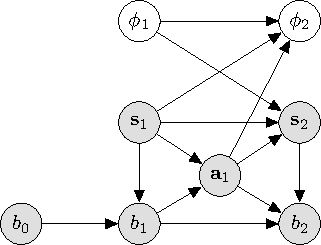
\includegraphics[width=0.5\linewidth]{figs/model.pdf}
\caption{Graphical model}
\end{subfigure}
\begin{subfigure}[b]{0.5\textwidth}
\centering
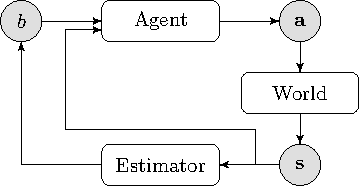
\includegraphics[width=0.5\linewidth]{figs/system_structure.pdf}
\caption{System structure}
\end{subfigure}
\end{figure*}

We assume that there exists a latent physics variable $\phi$ which determines the transition function of the underlying MDP, i.e., the transition function  $P(s',\phi' |s, \phi, a)$ is now a function of state, action, and $\phi$. We would like to learn a policy which maximizes the long term reward given $\phi$. Formally, this is called a Bayes-Adaptive MDP~\cite{ghavamzadeh2015bayesian, ross2008bayes, guez2012efficient}, defined by a tuple $\langle \mathcal{S}', \mathcal{A}, P, P_0, R \rangle$ where
\begin{itemize}
\item $\mathcal{S'} = \mathcal{S}\times \Phi$ is the set of hyper-states (states, physics variable),
\item $\mathcal{A}$ is the set of actions,
\item $P(s',\phi'|s, \phi, a)$ is the transition function between hyper-states, conditioned
on action $a$ being taken in hyper-state $(s, \phi)$,
\item $P_0\in \mathcal{P}(\mathcal{S} \times \Phi)$ combines the initial distribution over hyper-states,
\item $R(s, \phi, a)$ represents the reward obtained when action $a$ is
taken in hyper-state $(s,\phi)$.
\end{itemize}

We would like to find the Bayes-optimal policy for the following Bellman equaton:
\begin{equation}\label{eq:rl}
V^*(b, s) = \max_a \bigg\{R(b, s, a) + \gamma \sum_{s'}P(s'|b, s, a)V^*(b', s') \bigg\}.
\end{equation}
where $b$ is the belief over the set of latent physics parameters $\phi \in \Phi$.

We make a simplification to the BARL formulation. We assume that the latent variable $\phi$ is either constant or the rate of change is slow enough that approximating the long-term value with a determinized $\phi$ is a reasonable short-term approximation for choosing one-step action, i.e. we can treat $V^*(s_t, \phi_t) \approx V^*(s_t, \phi_{t:\infty})$ for the purpose of one-step Bellman update.

This assumption allows us to simplify BARL with an ensemble policy learning method. At a high level, we have a network that updates the \emph{belief} of the physics parameters at time $t$,
\begin{align*}
b(\phi_t) = P(\phi_t|s_{t-1}, \phi_{t-1}, a_{t-1})
\end{align*}
which is then used to compute the best policy from an ensemble of $\phi$-dependent optimal policies, i.e., $\pi^*(\cdot;\phi)$ and $V^*(\cdot;\phi)$ are computed with typical RL algorithms for MDPs. Then the remaining task is to compute the one-step best action $a$:
\begin{align}\label{eq:barl}
 a^* &= \argmax_{a} \mathbb{E}_{\phi \sim b(\phi)} \bigg[R(s, a, \phi) + \gamma \sum_{s', \phi'}P(s',\phi'|s, \phi, a)V^{*'}(s', \phi') \bigg].
\end{align}

The probability of an MDP $\mathcal{M}$, governed by latent physics variable $\phi_{\mathcal{M}}$, generating a trajectory $\tau$ is given by:
\begin{align}
P(\mathcal{M} | \tau) &= \frac{1}{Z}P(\tau | \mathcal{M}) \times P(\phi_\mathcal{M}) \nonumber \\
					  &= \frac{1}{Z}\prod_{t = 0}^{T-1}{P(s = s_{t+1}|s_t, a_t, \phi_\mathcal{M})} \times P(\phi_\mathcal{M})
\end{align}
where $Z$ is the normalizing constant that allows the sum of probabilities over all the MDPs to be unity. These probabilities are used to update the belief.

\subsection{Bayes-Adaptive Policy Network}

TODO: Explain how the system works (input to the network, etc.)
%%\newcommand{\argmin}{\operatornamewithlimits{\arg\min}}
%
%
%------------------------------------------
% Algorithm:
%------------------------------------------%
\begin{algorithm}[tb]
\caption{\texttt{Bayesian-DRL}}
\label{alg:highLevel}	
\begin{algorithmic}[1]
\State Statement and a comment. \Comment{Initialization}
\vspace{2mm}
\For{each statement in this for loop} \Comment{Hi there} 
	\State down a can of beer. :P
\EndFor
\State okie-dokey.
\While{JS is drawing his error bars}
	\State add text.
	\If{I mess up}
		\State Gilwoo will correct it ha!
	\Else
		\State we are screwed
	\EndIf   		
\EndWhile
\State \textbf{return} brian's awesome results.
\end{algorithmic}
\end{algorithm}

\section{Analysis}

\begin{itemize}
	\item By augmenting the observation with a belief over 	MDPs, policy networks can learn to be robust against 	model uncertainty while maintaining some of the
	``optimal'' actions w.r.t. each MDP.
	\item When the optimal policies across MDPs have a lot in 	common (e.g., Swimmer), simple "interpolation" of the deterministic policies provide good action proposals,
	suggesting that a mixture of policies (with a large number of policies that cover the space), may reduce sample complexity and offer even better performance.
\end{itemize}

\section{Results}

\begin{itemize}
	\item MuJoCo environments: Ant, Swimmer, HalfCheetah
	\begin{itemize}
		\item Uniformly sampled 20 MDPs across a range of parameters (e.g., body link length, mass, geometry size, joint damping, friction)
	\end{itemize}
	\item Algorithm Implementations:
	\begin{itemize}
		\item All policy networks were Gaussian MLPs with two layers, (64, 64), except for Bayes ones which had (128, 64) to account for the larger input space
		\item TRPO implementation from \texttt{rllab}
		\item EPOpt implemented based on the paper
		\item Bayes-Mixture Policy uses TRPO policies trained on the 20 MDPs to mix actions based on the belief
		\item QMDP uses TRPO policies trained on the 20 MDPs to rollout trajectories and approximate Q-functions
	\end{itemize}
\end{itemize}

\section{Future Work}

\begin{itemize}
	\item Extend to a continuous version which has Gaussian belief distribution as input
	\item Bootstrap a set of stochastic/deterministic policies, each trained for one MDP or a small range of parameters
	\item Train with additional reward bonus for information gain which helps distinguishing policies (not just beliefs)
\end{itemize}

%While reinforcement learning is capable of controlling complex autonomous systems, RL algorithms typically require huge amounts of data, can overfit to a particular task, or may learn brittle policies that are prone to disturbances. One of the main challenges that needs to be addressed is to train a policy that is robust to various model uncertainties and disturbances. In this project, we aim to address this challenge via an ensemble policy for Bayes-Adaptive Reinforcement Learning~\cite{ghavamzadeh2015bayesian}.
%
%We model $b_\phi$ as a network capable of modeling evolving state change, e.g., Recurrent Neural Networks, or as a Bayes filter. At the low level, we plan to discretize $\Phi$ and have one actor-critic network per discretized value of $\phi$: each critic estimates $V^*(\cdot;\phi)$ and each actor has an optimal policy for a particular discretized value of $\pi^*(\cdot;\phi)$. Given $b_\phi$ and the set of value-function approximators, it is straightforward to compute (\ref{eq:barl}).

\section{Related Works}

\newpage

%\begin{algorithm}[t!]
% \KwData{this text}
% \KwResult{how to write algorithm with \LaTeX2e }
% initialization\;
% \While{not at end of this document}{
%  read current\;
%  \eIf{understand}{
%   go to next section\;
%   current section becomes this one\;
%   }{
%   go back to the beginning of current section\;
%  }
% }
% \caption{TODO: write the algoruthm. (Change this to a prettier algorithm package)}
%\end{algorithm}

\section{Experiments}

We have setup a set of simulated examples and a set of RL algorithms to be utilized in our ensemble approach. For simulated examples, we have the following agents: \textbf{ant, reacher, swimmer, half-cheetah}, each with a predefined reward function defined similar to those given by OpenAI Gym~\cite{openai}. We are utilizing TRPO~\cite{trpo}, VPG, DDPG~\cite{ddpg} provide by \texttt{rllab}~\cite{duan2016benchmarking} as a set of algorithms to be utilized in our ensemble approach. In addition, we plan to implement PPO and a PID controller for RACECAR.

Our algorithm will be compared against two classes of algorithms: (1) sample-based algorithms which chooses an MDP and commit to this policy for a fixed horizon, and (2) ensemble algorithms which train a policy over an ensemble of MDP models. A greedy algorithm which chooses the maximum-likely MDP, or one that samples from a posterior distribution of MDPs given previous observations (e.g. Posterior Sampling Reinforcement Learning \cite{psrl}) would fall into the former, and EPOpt\cite{rajeswaran2016epopt} and Ensemble-CIO~\cite{ensemble-cio} would fall into the latter.

We are currently in the process of setting up baseline algorithms which may be used for direct comparison or as internal policy update algorithms for each of MDP in our algorithm.

\newpage
\begin{figure*}[t!]
\begin{centering}
\begin{subfigure}[b]{0.3\columnwidth}
\adjincludegraphics[height=3cm,trim={{.6\width} {0.4\height} {0.15\width} {0.35\height}},clip=true]{figs/keyframes/cheetah/cheetah_nominal.png}
\caption{Nominal}
\end{subfigure}
\begin{subfigure}[b]{0.3\columnwidth}
\adjincludegraphics[height=3cm,trim={{.5\width} {0.4\height} {0.25\width} {0.35\height}},clip=true]{figs/keyframes/cheetah/cheetah_170_92.png}
\caption{Key frames}
\end{subfigure}
\begin{subfigure}[b]{0.3\columnwidth}
\adjincludegraphics[height=3cm,trim={{.5\width} {0.4\height} {0.25\width} {0.35\height}},clip=true]{figs/keyframes/cheetah/cheetah_150_150.png}
\caption{Key frames}
\end{subfigure}
\end{centering}
\caption{Keyframes from rollouts on various MDPs. The universal policy network learns to use different policies on different MDPs.}
\end{figure*}


\newpage
\begin{figure*}[t!]
\begin{centering}
\begin{subfigure}[b]{0.38\columnwidth}
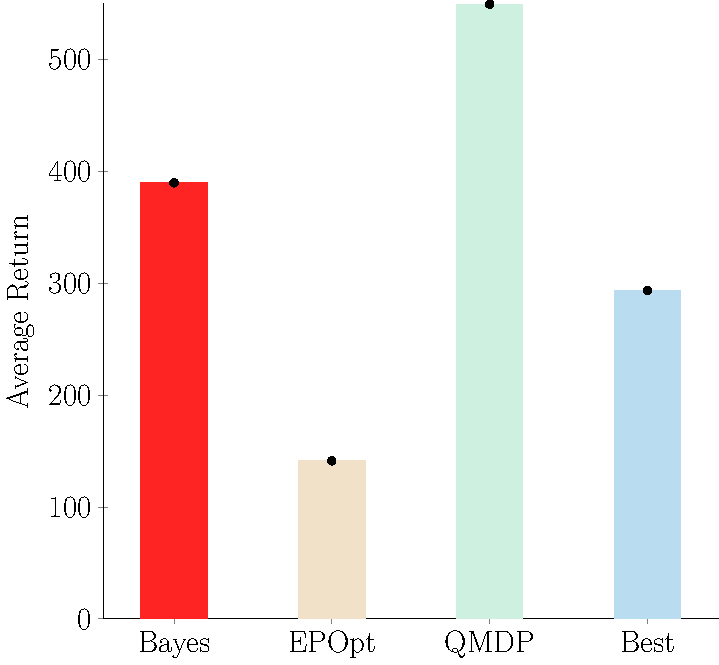
\includegraphics[width=\linewidth]{figs/cheetah_nominal_comparison.pdf}
\subcaption{Return on a sampled MDP}
\end{subfigure}
~
\begin{subfigure}[b]{0.38\columnwidth}
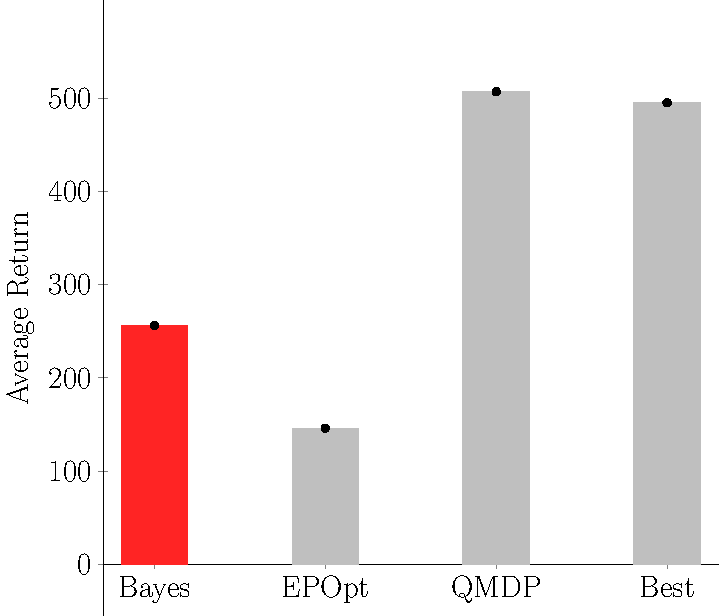
\includegraphics[width=\linewidth]{figs/cheetah_env_comparison.pdf}
\subcaption{Return on one of the chosen MDPs}
\end{subfigure}
~
\begin{subfigure}[b]{0.20\columnwidth}
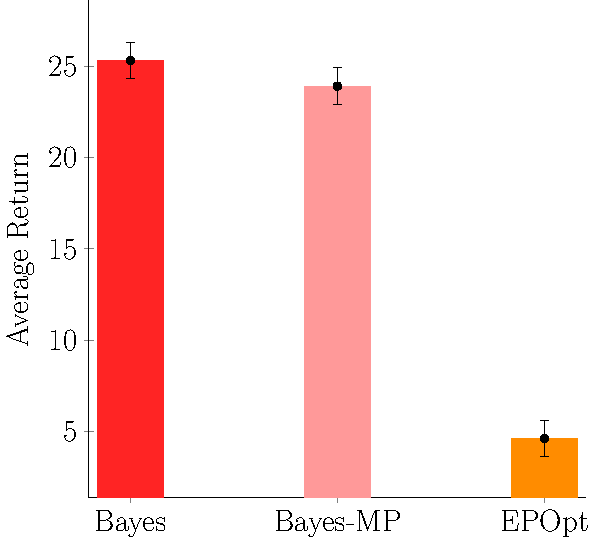
\includegraphics[width=\linewidth]{figs/ant_average.pdf}
\subcaption{Average return}
\end{subfigure}
\end{centering}
\caption{Return on sampled and prechosen MDPs. BARL is better than EPOpt. On average across K pre-chosen MDPs, it outperforms EPOpt by a large margin. TODO: remove BMP.}
\end{figure*}

\begin{figure*}[t!]
\begin{centering}
\begin{subfigure}[b]{0.38\columnwidth}
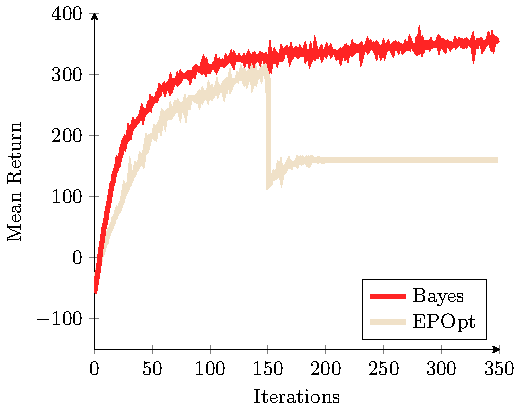
\includegraphics[width=\linewidth]{figs/cheetah_training_curves.pdf}
\subcaption{Return on a sampled MDP}
\end{subfigure}
~
\begin{subfigure}[b]{0.38\columnwidth}
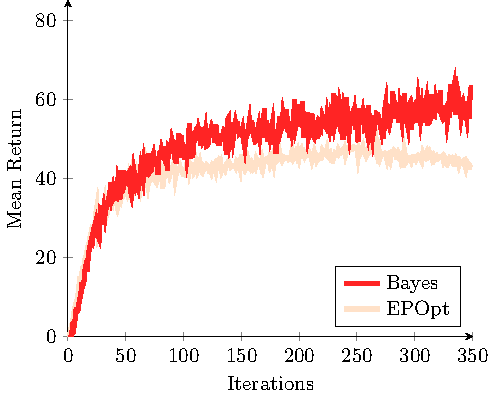
\includegraphics[width=\linewidth]{figs/swimmer_training_curves.pdf}
\end{subfigure}
\end{centering}
\caption{Training curves}
\end{figure*}



\newpage
\begin{figure*}[t!]
\begin{centering}
\begin{subfigure}[b]{0.3\columnwidth}
\adjincludegraphics[height=3cm,trim={{.4\width} {0.42\height} {0.35\width} {0.33\height}},clip=true]{figs/keyframes/ant/ant_nominal_18.png}
\caption{Nominal}
\end{subfigure}
\hfill
\begin{subfigure}[b]{0.3\columnwidth}
\adjincludegraphics[height=3cm,trim={{.4\width} {0.42\height} {0.35\width} {0.33\height}},clip=true]{figs/keyframes/ant/ant_120_19.png}
\caption{Key frames}
\end{subfigure}
\hfill
\begin{subfigure}[b]{0.3\columnwidth}
\adjincludegraphics[height=3cm,trim={{.6\width} {0.34\height} {0.15\width} {0.41\height}},clip=true]{figs/keyframes/ant/ant_140_87.png}
\caption{Key frames}
\end{subfigure}
\vfill
\begin{subfigure}[b]{0.3\columnwidth}
\adjincludegraphics[height=3cm,trim={{.55\width} {0.34\height} {0.20\width} {0.41\height}},clip=true]{figs/keyframes/swimmer/swimmer_nominal.png}
\caption{Nominal}
\end{subfigure}
\hfill
\begin{subfigure}[b]{0.3\columnwidth}
\adjincludegraphics[height=3cm,trim={{.55\width} {0.40\height} {0.20\width} {0.35\height}},clip=true]{figs/keyframes/swimmer/swimmer_20_12.png}
\caption{Key frames}
\end{subfigure}
\hfill
\begin{subfigure}[b]{0.3\columnwidth}
\adjincludegraphics[height=3cm,trim={{.35\width} 0 {0.40\width} {0.55\height}},clip=true]{figs/keyframes/swimmer/swimmer_40_157.png}
\caption{Key frames}
\end{subfigure}
\caption{Keyframes from rollouts on various MDPs. Some of the MDPs are gemeotrically significatnly differnt that they require drastically different policies to achieve optimal returns.}
\end{centering}
\end{figure*}

\bibliography{intuitive_physics}

\end{document}
